\section{容器、迭代器和算法的设计}
容器是表示元素集合的类型。这些集合可以基于各种数据结构实现,每种结构都具有不同的语义:列表、队列、树等等。标准库提供了三类容器:

\begin{itemize}
  \item
        序列容器:vector、deque、list、array和forward\_list

  \item
        关联容器:set、map、multiset和multimap

  \item
        无序关联容器:unordered\_set、unordered\_map、unordered\_multiset和unordered\_multimap
\end{itemize}

除此之外,还有为序列容器提供不同接口的容器适配器。这个类别包括堆stack、queue和priority\_queue类。最后,还有一个名为span的类,表示连续对象序列上的非所属视图。

将这些容器作为模板的基本原理,已经在第1章模板介绍中介绍过。因为不希望为需要存储在容器中,每种不同类型的元素一次又一次地编写相同的实现。标准库中最常用的容器如下:

\begin{itemize}
  \item
        vector: 一个连续存储在内存中的可变大小的元素集合。若没有定义特殊需求,是默认选择的容器。内部存储器根据需要自动扩展或收缩以容纳存储的元素。vector分配的内存比需要的多,因此需要扩展的风险很低。扩展是一项开销很大的操作,因为需要分配新的内存,需要将当前存储的内容复制到新存储中,最后需要丢弃之前的存储。因为元素连续地存储在内存中,所以索引可以在常数时间内随机访问。

  \item
        array: 连续存储在内存中的固定大小的元素集合,size必须是编译时常量表达式。数组类的语义与保存C风格数组(T[n])的结构相同。就像vector类型一样,数组类的元素可以在常数时间内随机访问。

  \item
        map: 将值关联到唯一键的集合。键用比较函数排序,map类通常实现为红黑树。搜索、插入或删除元素的操作具有对数(log(n))复杂度。

  \item
        set: 唯一键的集合。键是容器中存储的实际值,map类中没有键值对。就像map类一样,set通常也使用红黑树实现,在搜索、插入和删除元素时具有对数(log(n))复杂度。
\end{itemize}

不管它们的类型是什么,标准容器有一些共同点:

\begin{itemize}
  \item
        几种常见成员类型

  \item
        存储管理的分配器(除了std::array类)

  \item
        几个公共成员函数(其中一些在一个或另一个容器中缺失)

  \item
        迭代器可访问存储的数据
\end{itemize}

以下成员类型由所有标准容器定义:

\begin{cpp}
using value_type = /* ... */;
using size_type = std::size_t;
using difference_type = std::ptrdiff_t;
using reference = value_type&;
using const_reference = value_type const&;
using pointer = /* ... */;
using const_pointer = /* ... */;
using iterator = /* ... */;
using const_iterator = /* ... */;
\end{cpp}

这些别名的实际类型可能因容器而异。例如,对于std::vector, value\_type是模板参数T,但是对于std::map, value\_type是std::pair<const Key, T>类型。这些成员类型的目的是进行泛型编程。

除了std::array类(表示编译时已知大小的数组),其他所有容器都是动态分配内存的,可以通过分配器对象来控制的。其类型指定为类型模板形参,但若没有指定,则所有容器默认为std::allocator。这个标准分配器使用全局的new和delete操作符来分配和释放内存。标准容器的所有构造函数(包括复制和移动构造函数)允许指定分配器。

标准容器中还定义了一些常用的成员函数。下面是一些例子:

\begin{itemize}
  \item
        size, 返回元素的数量(std::forward\_list没有)。

  \item
        empty, 检查容器是否为空。

  \item
        clear, 清除容器的内容(std::array,std::stack,std::queue和std::priority\_queue中没有)。

  \item
        swap, 交换容器对象的内容。

  \item
        begin和end方法,返回到容器的开始和结束的迭代器(std::stack, std::queue和std::priority\_queue中没有,尽管这些不是容器,而是容器适配器)。
\end{itemize}

最后提到了迭代器。这些类型抽象了容器中访问元素的细节,提供了一种统一的方法来标识和遍历容器中的元素。这很重要,因为标准库的关键部分是由通用算法表示的。有超过一百种这样的算法,从序列操作(如count、count\_if、find和for\_each)到修改操作(如复制、填充、转换、旋转和反向)到分区和排序(分区、排序、nth\_element)等。迭代器是确保它们一般性工作的关键,若每个容器都有不同的方式访问其元素,那么编写泛型算法几乎是不可能的。

这里考虑将元素从一个容器复制到另一个容器的简单操作。例如,有一个std::vector对象,希望将其元素复制到std::list对象:

\begin{cpp}
std::vector<int> v {1, 2, 3};
std::list<int> l;

for (std::size_t i = 0; i < v.size(); ++i)
	l.push_back(v[i]);
\end{cpp}

若想从std::list复制到std::set,或者从std::set复制到std::array呢?每种情况都需要不同类型的代码。通用算法使能够以统一的方式完成:

\begin{cpp}
std::vector<int> v{ 1, 2, 3 };

// copy vector to vector
std::vector<int> vc(v.size());
std::copy(v.begin(), v.end(), vc.begin());

// copy vector to list
std::list<int> l;
std::copy(v.begin(), v.end(), std::back_inserter(l));

// copy list to set
std::set<int> s;
std::copy(l.begin(), l.end(), std::inserter(s, s.begin()));
\end{cpp}

这里有一个std::vector对象,将其内容复制到另一个std::vector对象,也复制到std::list对象。因此,std::list对象的内容随后复制到std::set对象。对于所有情况,都可以使用std::copy算法。该算法有几个参数:两个迭代器定义源的开始和结束,一个迭代器定义目标的开始。该算法通过输出迭代器每次从输入范围复制一个元素到元素指针,然后对输出迭代器进行递增。可以实现的方式如下所示:

\begin{cpp}
template<typename InputIt, class OutputIt>
OutputIt copy(InputIt first, InputIt last,
			  OutputIt d_first)
{
	for (; first != last; (void)++first, (void)++d_first)
	{
		*d_first = *first;
	}
	return d_first;
}
\end{cpp}

\begin{important}
  该算法在第5章中讨论过,当时我们研究了如何利用类型特征优化其实现。
\end{important}

考虑到前面的例子,有些情况下,目标容器的内容还没有分配以便进行复制。这是复制到列表和复制到集合的情况。类似迭代器的类型std::back\_insert\_iterator和std:insert\_iterator,通过std::back\_inserter和std::inserter辅助函数间接使用,用于将元素插入容器中。std::back\_insert\_iterator类使用push\_back函数,std::insert\_iterator类使用insert函数。

C++中有六种迭代器类型:

\begin{itemize}
  \item
        输入迭代器

  \item
        输出迭代器

  \item
        前向迭代器

  \item
        双向迭代器

  \item
        随机迭代器

  \item
        连续迭代器
\end{itemize}

连续迭代器是在C++17中添加的。所有操作符都可以使用前缀或后缀增量操作符进行递增。下表显示了每个类别定义的操作:

\begin{longtblr}
  { colspec = {|c|X[2]|X[1]|}, hlines, rowhead = 1, rows={m}, row{1} = {c, font=\bfseries} }
  类别                  & 属性                & 表达式               \\
  \SetCell[r=3]{c} 输入
                      & 单次增加              & {i++              \\ ++i}              \\
                      & 相等/不相等的比较         & {i == j           \\ i != j}        \\
                      & 可以解引用(作为右值)       & {*i               \\ i-\textgreater{}m} \\
  前向                  & 多次增加              & {i = j, *j++, *i} \\
  双向                  & 可减                & {--i              \\ i--}              \\
  \SetCell[r=4]{c} 随机
                      & 算术运算符+和-          & {i + n            \\ n + i\\ i - n\\ n - i} \\
                      & 不等式比较(使用迭代器)      & {i \textless j    \\ i \textgreater j\\ i \textless{}= j\\ i \textgreater{}= j} \\
                      & 复合赋值              & {i += n           \\ i -= n}        \\
                      & 偏移解引用操作符          & i{[}n{]}          \\
  连续                  & 逻辑上相邻的元素,内存物理上相邻。 &                   \\
  \SetCell[r=2]{c} 输出 & 单次增加              & {i++              \\ ++i}              \\
                      & 可以解引用(作为左值)       & {*i = v           \\ *i++ = v}      \\
\end{longtblr}

除了输出类别外,每个类别都有相关的内容。所以前向迭代器是输入迭代器,双向迭代器是前向迭代器,随机迭代器是双向迭代器。最后,连续迭代器是随机访问迭代器。前五种类型的迭代器,也可以同时是输出迭代器。这样的迭代器称为可变迭代器。否则,称为常量迭代器。

C++20标准增加了对概念和概念库的支持。这个标准库为每个迭代器类别定义了标准概念。它们之间的相关性如下表所示:

\begin{table}[!htb]
  \centering
  \begin{talltblr}
    { colspec = {|l|l|}, hlines, row{1} = {c, font=\bfseries} }
    迭代器类型 & 概念                            \\
    输入迭代器 & std::input\_iterator          \\
    前向迭代器 & std::output\_iterator         \\
    双向迭代器 & std::bidirectional\_iterator  \\
    随机迭代器 & std::random\_access\_iterator \\
    连续迭代器 & std::contiguous\_iterator     \\
    输出迭代器 & std::output\_iterator         \\
  \end{talltblr}
\end{table}

所有容器都有以下成员:

\begin{itemize}
  \item
        begin: 返回一个指向容器开头的迭代器。

  \item
        end: 返回一个指向容器末尾的迭代器。

  \item
        cbegin: 返回一个指向容器开头的常量迭代器。

  \item
        cend: 返回一个指向容器末端的常量迭代器。
\end{itemize}

一些容器也有返回反向迭代器的成员:

\begin{itemize}
  \item
        rbegin: 返回一个指向反向容器开头的反向迭代器。

  \item
        rend: 返回一个指向反向容器末尾的反向迭代器。

  \item
        rcbegin: 返回一个指向反向容器开头的常量反向迭代器。

  \item
        rcend: 返回一个常量反向迭代器,指向反向容器的末尾。
\end{itemize}

要使用容器和迭代器,需要理解两点:

\begin{itemize}
  \item
        容器的末尾不是容器的最后一个元素,而是在最后一个元素之后的元素。

  \item
        反向迭代器以相反的顺序提供对元素的访问,指向容器第一个元素的反向迭代器实际上是非反向容器的最后一个元素。
\end{itemize}

为了更好地理解这两点,来看看下面的例子:

\begin{cpp}
std::vector<int> v{ 1,2,3,4,5 };

// prints 1 2 3 4 5
std::copy(v.begin(), v.end(),
		  std::ostream_iterator<int>(std::cout, " "));

// prints 5 4 3 2 1
std::copy(v.rbegin(), v.rend(),
		  std::ostream_iterator<int>(std::cout, " "));
\end{cpp}

对std::copy的第一个调用以给定的顺序打印容器的元素。另一方面,对std::copy的第二次调用以相反的顺序打印元素。

对std::copy的第一个调用以给定的顺序打印容器的元素。另一方面,对std::copy的第二次调用以相反的顺序打印元素。

\begin{center}
  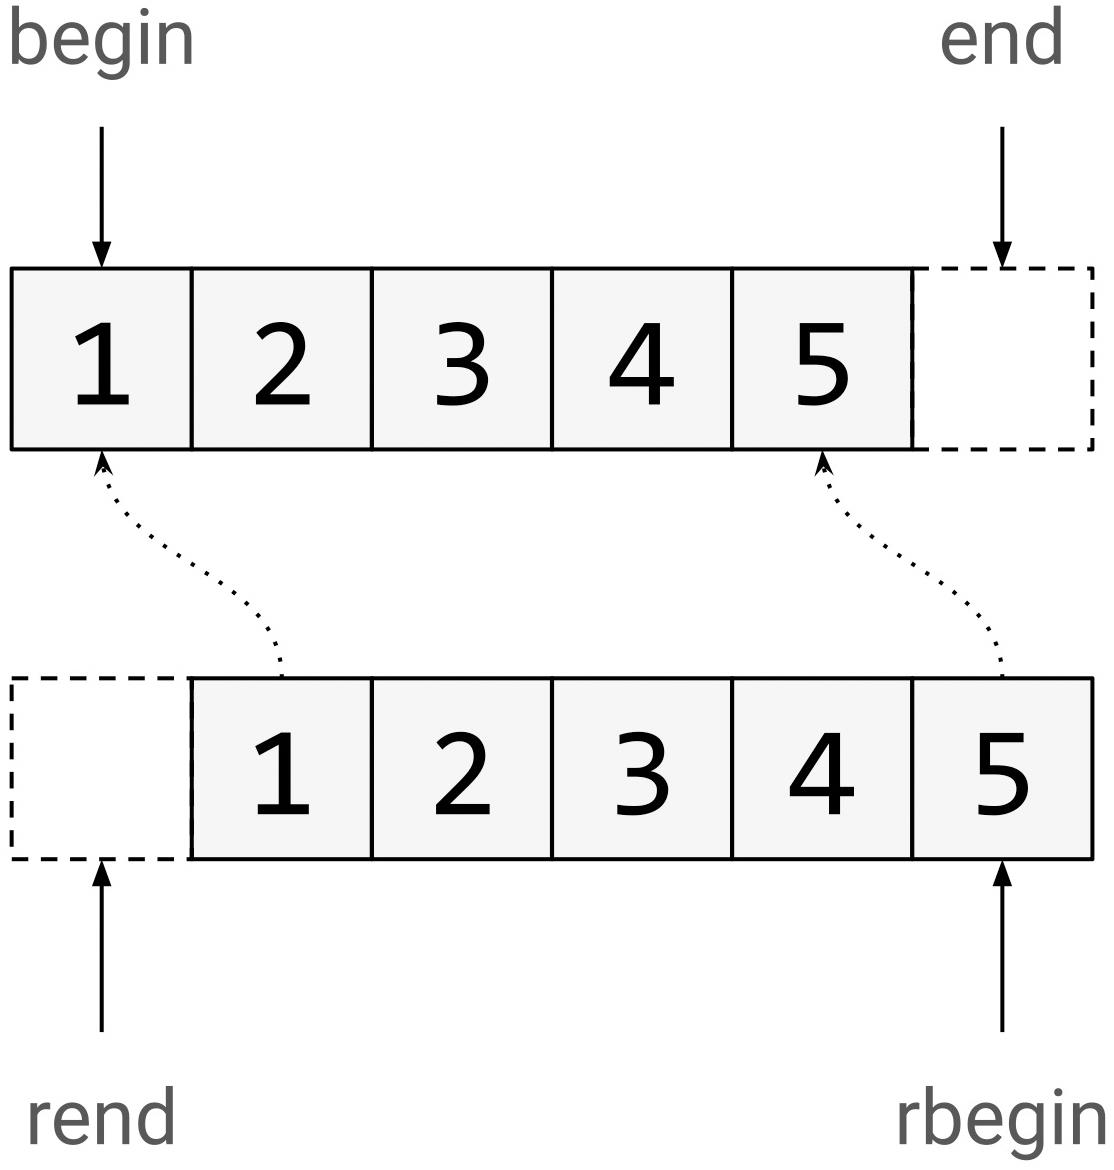
\includegraphics[width=0.4\textwidth]{images/1.png}\\
  图 8.1
\end{center}

两个迭代器(begin和end,即最后一个元素后面的那个)分隔的元素序列(不管它们在内存中存储的是什么样的数据结构)称为范围。这个术语在C++标准(尤其是算法)和文献中被广泛使用,也是C++20中范围库的名称,该库将在第9章中讨论。

除了标准容器的begin/end成员函数集合外,还有同名的独立函数。其等价性如下表所示:

\begin{table}[!htb]
  \centering
  \begin{talltblr}
    { colspec = {|l|l|}, hlines, row{1} = {c, font=\bfseries} }
    成员函数        & 独立函数            \\
	{c.begin() \\ c.cbegin()} & {std::begin(c) \\ std::cbegin(c)} \\
	{c.end() \\ c.cend()} & {std::end(c) \\ std::cend(c)} \\
	{c.rbegin() \\ c.crbegin()} & {std::rbegin(c) \\ std::crbegin(c)} \\
	{c.rend() \\ c.crend()} & {std::rend(c) \\ std::crend(c)} \\
  \end{talltblr}
\end{table}

尽管这些独立函数在使用标准容器时没有带来太多好处,但因为所有这些独立函数对于静态数组都是重载的,其有助于我们编写既可以处理标准容器,又可以处理类C数组的泛型代码。这里有一个例子:

\begin{cpp}
std::vector<int> v{ 1,2,3,4,5 };
std::copy(std::begin(v), std::end(v),
		  std::ostream_iterator<int>(std::cout, " "));

int a[] = { 1,2,3,4,5 };
std::copy(std::begin(a), std::end(a),
		  std::ostream_iterator<int>(std::cout, " "));
\end{cpp}

若没有这些函数,将要写成std::copy(a, a + 5,...),也许这些函数的好处是,使我们能够使用基于范围的for循环的数组:

\begin{cpp}
std::vector<int> v{ 1,2,3,4,5 };
for (auto const& e : v)
	std::cout << e << ' ';

int a[] = { 1,2,3,4,5 };
for (auto const& e : a)
	std::cout << e << ' ';
\end{cpp}

本书的目的不是教你如何使用每个容器或许多标准算法,但学习如何创建容器、迭代器和算法应该是有帮助的。这就是我们接下来要做的。
